
\documentclass[10pt,a4paper,titlepage]{article}
\usepackage[english]{babel}
\usepackage[utf8]{inputenc}
\usepackage[margin=100pt]{geometry}


\usepackage{graphicx}   % Import pictures
\usepackage{ragged2e}   % fullfill paragraphs
%\usepackage{multicol}
%\usepackage{lscape}
\usepackage{xcolor}
%\usepackage{listings}
\usepackage{courier}
\usepackage{caption}

\usepackage[backend=biber]{biblatex}
\addbibresource{dokumentace.bib}



\begin{document}
%-----------------------------------------%
%	            TITLE PAGE                %
%-----------------------------------------%
\begin{titlepage}

\begin{center}
% Headings
\textsc{\LARGE Brno University of technology}\\[0.5cm]
\textsc{\large Faculty of Information Technology}\\[8cm]

% Title - lines
{ \huge \bfseries IPK project 2}\\[0.3cm]
{ \Large \bfseries documentation}\\[0.5cm]
{ \bfseries Martin Benes}\\

\end{center}

\end{titlepage}
\newpage

%-----------------------------------------%
%	              DOCUMENT                  %
%-----------------------------------------%

\pagenumbering{gobble}

The task of the project was to gather informations about DHCP protocol and afterwards write a program in C,
that performs a DHCP starvation attack.

\section*{DHCP}

\subsection*{Motivation}
Every private network manages its own IP address space with reserved addresses, that
can be given to the internal devices. The assignment of the addresses may be
done either manually or automatically, using DHCP agent.

Manual configuration forces the network administrator to manually setup the
IP for each device, newly connected to the network. On the other hand, there
is also a possibility of automatic assignment, using DHCP protocol.

It requires to have a special program, running on some local address. The program
has a pool of available addresses in the network and when the new device
appears, it will communicate with it and assigns an local IP address to it.


\subsection*{DHCP protocol}

\begin{figure}[h!]
    \begin{center}
        \includegraphics[width=0.2\textwidth]{dhcpcomm.png}
        \caption{ DHCP communication. \label{fig:triangle} \cite{DHCPcomm}}
    \end{center}
\end{figure}

When the new device shows up in the network, it may not receive any addresses,
because the sender would not be able to set a destination IP, because the
device does not have any.

The device has to inform DHCP server about itself. The DHCP server does not have
any strict local address, so the device sends {\it DHCP Discovery} packet to the
broadcast address {\it ff.ff.ff.ff}, which is received by every device in the
network, including the DHCP server.

The server then reserves an address for the device, and sends {\it DHCP Offer}
response, unicast or multicast (set in received DHCP Discovery). If the
unicast is used, the MAC address from the DHCP Discovery is used as target
address (on L2).

The DHCP client (the device) then sends {\it DHCP Request} to the server (again
it must be to the broadcast address, the local address is not assigned yet).
The client may receive several DHCP Offer packets (there might be more DHCP
servers in the network), but when the servers receives the DHCP Request from
the client, answering another server, they will withdraw the offer and return
the reserved address back to the address pool.

After receiving the DHCP Request, the process comes to its final phase. The server
sends {\it DHCP Acknowledgement}, including address lease duration.
\cite{DHCPwikipedia}



\printbibliography

\end{document}